\subsection{多面体的变形}\label{subsec:3-4}
\begin{enhancedline}

我们考虑任意一个多面体,例如正六面体,假定它的面是用橡胶薄膜做成的。
如果充以气体,那么它就会连续(不破裂)变形,最后可变为一个球面(图 \ref{fig:ltjh-3-11})。

\begin{figure}[htbp]
    \centering
    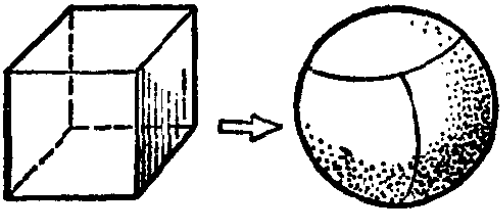
\includegraphics[width=6cm]{../pic/ltjh-ch3-11.png}
    \caption{}\label{fig:ltjh-3-11}
\end{figure}

象这样,表面连续变形,可变形为球面的多面体叫做\zhongdian{简单多面体}。
棱柱、棱锥、棱台、正多面体、凸多面体都是简单多面体。

除简单多面体外,还有不是简单多面体的几何体,例如将正方体挖去一个洞所得的几何体(图 \ref{fig:ltjh-3-12})。
这样的几何体的表面连续变形后就不能变为一个球面,而能变为一个环面。

\begin{figure}[htbp]
    \centering
    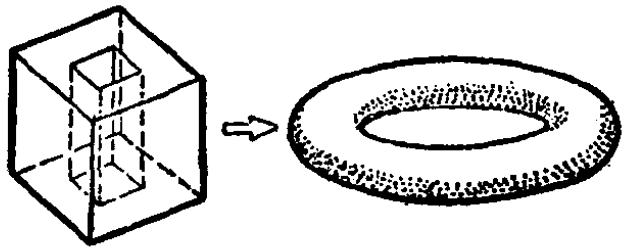
\includegraphics[width=7cm]{../pic/ltjh-ch3-12.png}
    \caption{}\label{fig:ltjh-3-12}
\end{figure}

我们曾研究过五种正多面体,发现它们的顶点数 $V$、棱数 $E$ 和面数 $F$ 有下面关系:
$$ V + F - E = 2 \juhao $$
现在用连续变形的方法研究简单多面体,看它的顶点数 $V$、棱数 $E$ 和面数 $F$ 是否也有这种关系。
以四面体 $ABCD$ 为例,将它的一个面 $BCD$ 去掉,再使它变形为平面图形(图 \ref{fig:ltjh-3-13})。
\begin{figure}[htbp]
    \centering
    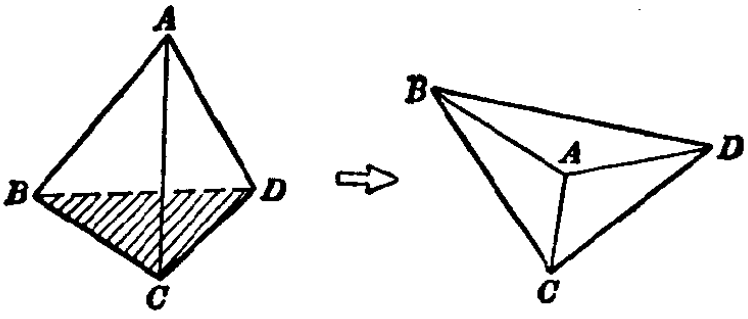
\includegraphics[width=9cm]{../pic/ltjh-ch3-13.png}
    \caption{}\label{fig:ltjh-3-13}
\end{figure}
这时,四面体的顶点数 $V$、棱数 $E$ 与剩下的面数 $F_1$,变形后都没有变。
因此,要研究 $V$、$E$、$F$ 之间的关系,研究平面图形即可。我们来研究
$$ V + F_1 - E $$
的数值。可按下面两步进行:

1. 去掉一条棱,就减少一个面,例如去掉 $BC$,就减少一个面 $ABC$。
同理,去掉棱 $CD$、$BD$ 时,也都随着各减少一个面 $ACD$、$ABD$(图 \ref{fig:ltjh-3-14}),
由于 $F_1 - E$、$V$的值都不变,因此,$V + F_1 - E$ 的值不变。

\begin{figure}[htbp]
    \centering
    \begin{minipage}[b]{7cm}
        \centering
        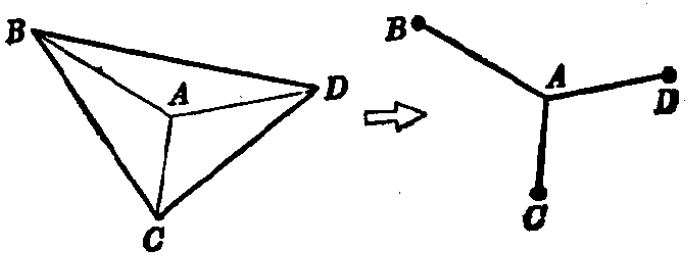
\includegraphics[width=7cm]{../pic/ltjh-ch3-14.png}
        \caption{}\label{fig:ltjh-3-14}
    \end{minipage}
    \qquad \qquad
    \begin{minipage}[b]{7cm}
        \centering
        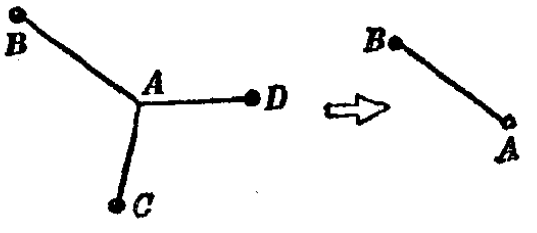
\includegraphics[width=6cm]{../pic/ltjh-ch3-15.png}
        \caption{}\label{fig:ltjh-3-15}
    \end{minipage}
\end{figure}

2. 再从剩下的树枝形,去掉一条棱,就减少一个顶点。
例如去掉 $CA$,则减少一个顶点 $C$。
同理,去掉棱 $DA$ 随着减少一个顶点 $D$,最后剩下 $AB$(图 \ref{fig:ltjh-3-15})。
在此过程中 $V - E$ 的值都不变。
但这时因为面数 $F_1$ 都是 $0$,所以,$V + F_1 - E$ 的值也不变。
由于最后只剩下 $AB$,因此
$$ V + F_1 - E = 2 + 0 - 1 = 1 \juhao $$

最后,加上最初去掉的一个面,得到
$$ V + F - E = 2 \juhao $$

因为对任意的简单多面体,应用这样的方法,最后都是只剩一条线段,
因而都得到上面的结果,所以可以把它写成下面的定理:

\begin{dingli}[定理][dl:eldl]
    简单多面体的顶点数 $\bm{V}$、棱数 $\bm{E}$、面数 $\bm{F}$,有下面的关系
    \begin{center}
        \framebox[12em]{$\bm{V + F - E = 2}$。}
     \end{center}
\end{dingli}

这个定理叫做\zhongdian{欧拉定理}。 它表明 2 这个数是简单多面体表面在连续变形下不变的数。


\liti[0] 一个简单多面体的面都是三角形。求证: $F = 2V - 4$。

\zhengming 因为已知多面体的每个面有三条边,每相邻两个面的两条边重合为一条棱,
所以棱数 $E = \dfrac{3F}{2}$,代入公式 $V + F - E = 2$,得
$$ V + F - \dfrac{3F}{2} = 2 \juhao $$
化简得
$$ F = 2V - 4 \juhao $$


\begin{lianxi}

\xiaoti{检查六棱柱、五棱锥、四棱台,看它们的顶点数、棱数、面数是否适合欧拉定理。}

\xiaoti{简单多面体、凸多面体、正多面体、棱柱、棱锥、棱台的包含关系如何?用图表示。}

\end{lianxi}
\end{enhancedline}
